% Provenance (never printed): see sources/outline_sources.md (Year 1: field
% notebook, compass-clinometer, hand lens, sampling, polarising microscope and
% thin sections, safety). The readings of the Varden east limb are simulated
% in figdata/bachelor-1/attitude_stats.py (seed 83, errors of 3 degrees);
% problem values in the Book 3 scratch calculator calc/ch06.py.
\chapter{طرائق الحقل والمختبر I}\label{ch:b1:field-lab-methods-1}

تحمل الجيولوجية التي ترسم خريطة تلال فاردن القليل: دفتر ملاحظات، وقلمًا رصاصيًا، ومستقبِل أقمار صناعية، وبوصلة مع مقياس الميل، وعدسة يدوية، وأكياسًا قليلة للعينات. وبهذه الأدوات تحدّد موضع وقوفها، وتقيس \omterm{def:b1:geological-maps:attitude}{وضعية} الطبقات، وتسمّي الصخور، وتعود بالعينات التي سيقطعها المختبر ويطحنها ويفحصها بالمجهر. وكل عدد في الفصول السابقة --- \omterm{def:b1:geological-maps:attitude}{وضعية} على خريطة، أو انحدار في مقطع --- بدأ قراءةً من هذا النوع، وله خطؤه الخاص. يصف هذا الفصل كيف يُجري المحترفون هذه المشاهدات، وكيف تُعدّ القراءات المتكررة ويُحوَّل تشتتها إلى عدم يقين. ويختم بموسم من القراءات على الجناح الشرقي \omterm{def:b1:geological-maps:fold}{لطية} فاردن.

\begin{recall}
تُكتب \omterm{def:b1:geological-maps:attitude}{وضعية المستوي} على صورة \omterm{def:b1:geological-maps:attitude}{اتجاه الانحدار}/\omterm{def:b1:geological-maps:attitude}{الانحدار}، مثل $081/12$، أو على صورة امتداد وفق قاعدة اليد اليمنى مع انحدار (\cref{ch:b1:geological-maps}). والانحراف المغناطيسي هو الزاوية بين الشمال الجغرافي والاتجاه الذي تشير إليه إبرة البوصلة (الفيزياء، الصف 11). ويُعرَف الصخر في اليد من بريقه وانشقاقه وصلابته ولونه (الكتاب 2، الصف 11). ويلخّص الوسط الحسابي والانحراف المعياري لمجموعة من الأعداد مركزها وتشتتها (الرياضيات).
\end{recall}

\section{الدفتر والخريطة}

\begin{definition}[محطة حقلية، ودفتر الحقل]\label{def:b1:field-lab-methods-1:station}
\emph{المحطة الحقلية}\index{المحطة الحقلية} مكان مرقّم يسجّل فيه الجيولوجي ملاحظاته: موضعه، والصخور المرئية، ووضعيتها، والعينات المأخوذة. و\emph{دفتر الحقل}\index{دفتر الحقل} هو السجلّ المجلّد للمحطات، بحسب ترتيب زيارتها، مع أرقامها ورسومها وقياساتها، مكتوبةً في الموقع نفسه.
\end{definition}

الدفتر هو السجلّ الأولي: ما لا يُكتب في المحطة يضيع، والخريطة التي تُرسم في المساء لا تعدو أن تكون بجودة الملاحظات التي وراءها. ولكل محطة رقم يظهر على الخريطة الحقلية، وفي الدفتر، وعلى كل كيس عينة أُخذت منها. والرسم يُظهر ما لا تُظهره قائمة من الأرقام --- كيف تلتقي وحدتان، وفي أيّ اتجاه تقع الطبقات الأحدث، وأين أُخذت قراءة على سطح مطوي --- ويسجّل مقياسه واتجاهه. وتُفصل الوقائع عن التفسيرات: مثل "حجر جيري فوق الصخر الطيني، \omterm{def:b1:geological-maps:geological-map}{والتماس} حادّ" ملاحظة؛ أما "عدم توافق" فاستنتاج يُكتب على هذا الأساس.

\begin{inthefield}[يوم في الرسم الخريطي]
% ledger: gps:smartphone-accuracy, gps:high-end
\begin{minipage}[t]{0.58\linewidth}\vspace{0pt}
يخطّط الجيولوجي الذي يرسم الخريطة مسارًا عبر \omterm{def:b1:geological-maps:attitude}{الامتداد}، ليلتقي كل وحدة بالتتابع، ويتوقف حيثما يظهر \omterm{def:b1:geological-maps:geological-map}{تماس} أو تغيّر في الصخر أو سطح قابل للقياس. وعند كل محطة يكتب رقمها وموضعها، ويرسم ما يراه، ويقيس الوضعيات، ويدوّن العينات. وتأتي المواضع من مستقبِل أقمار صناعية: فالمستقبِل العادي، مثل مستقبِل الهاتف الذكي، يكون دقيقًا عادةً ضمن نحو \qty{4.9}{m} في السماء المفتوحة، وأسوأ قرب الجروف والأشجار، بينما تبلغ المستقبِلات المساحية التي تستعمل تردّدين أو خدمات تصحيح بضعة سنتيمترات. وعند مقياس خريطة 1:10\,000 تكون \qty{4.9}{m} نصف مليمتر: فالمستقبِل العادي كافٍ للرسم الخريطي، لكنه لا يكفي لقياس الحركة البطيئة للأرض (\cref{ch:b1:plate-kinematics}).
\end{minipage}\hfill
\begin{minipage}[t]{0.39\linewidth}\vspace{0pt}
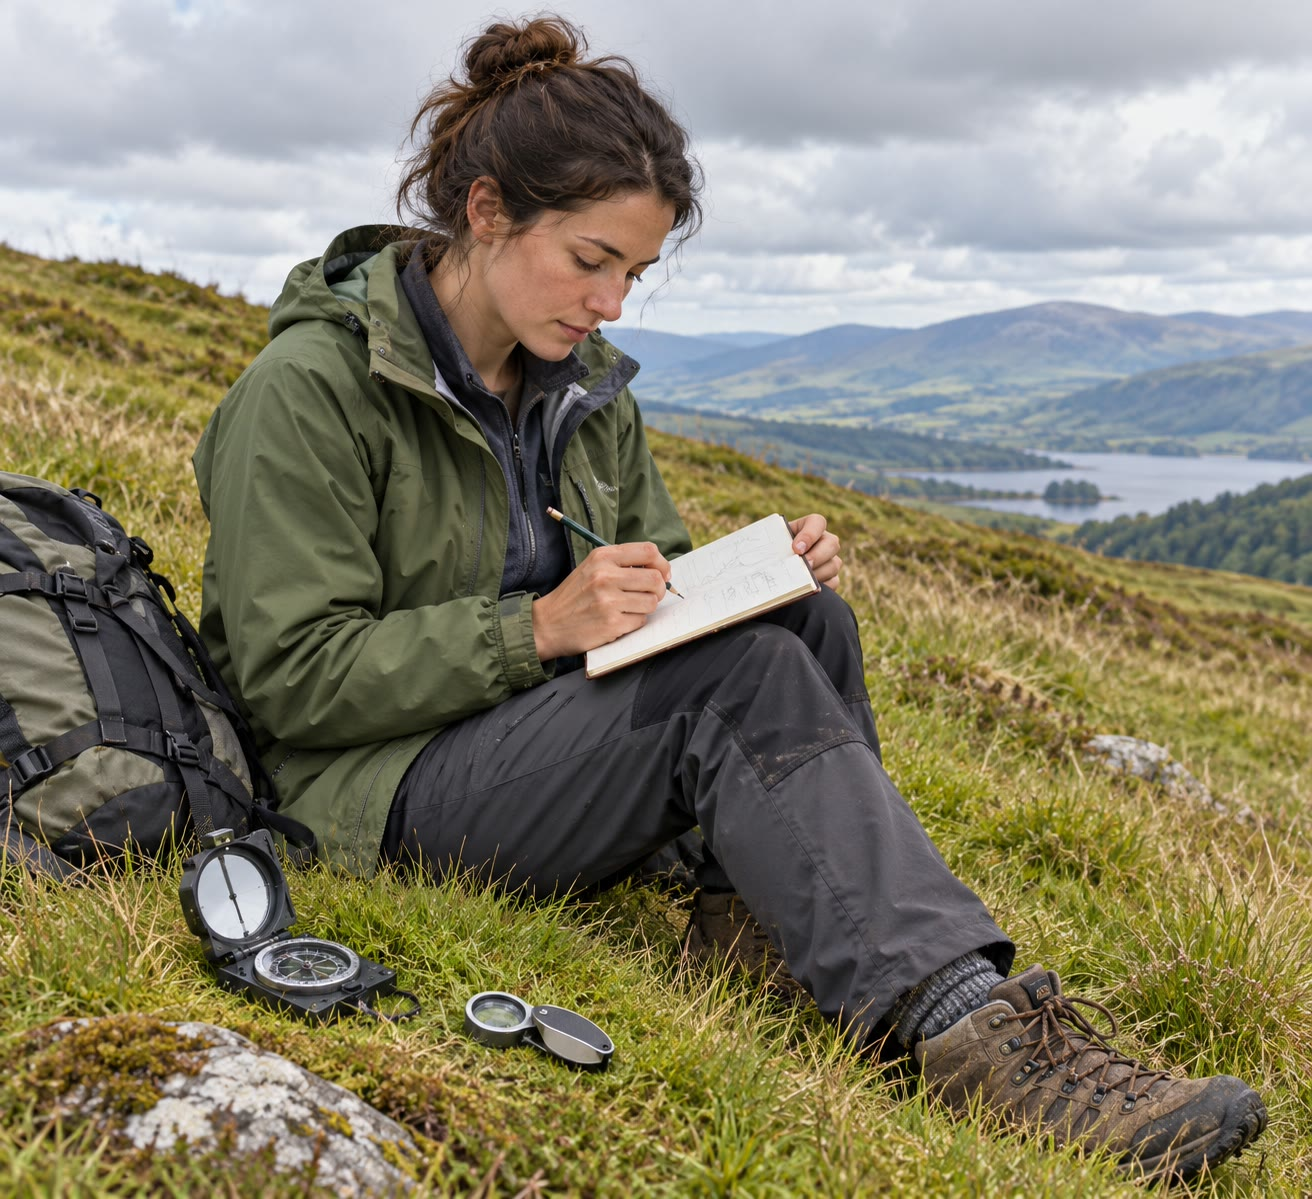
\includegraphics[width=\linewidth]{images/book3/ai/b1-field-notebook.jpg}
\end{minipage}
\end{inthefield}

\section{قياس الاتجاهات}

تُقاس \omterm{def:b1:geological-maps:attitude}{وضعية المستوي} --- طبقة، أو صدع، أو فاصل --- بالبوصلة ومقياس الميل: فالبوصلة المغناطيسية تقرأ \omterm{def:b1:spherical-astronomy:horizontal}{السمت}، ومِنْ بندول أو ميزان مستوٍ تُقرأ الزوايا عن الأفق. ويُوضع حرفها على امتداد السطح لتُقرأ \omterm{def:b1:geological-maps:attitude}{الامتداد}، أو تُوضع الأداة على السطح على طول خطه الأشدّ انحدارًا لتُقرأ \omterm{def:b1:geological-maps:attitude}{الانحدار}، ومن سمت ذلك الخط يُقرأ \omterm{def:b1:geological-maps:attitude}{اتجاه الانحدار}.

\begin{omfigure}
\begin{tikzpicture}[font=\scriptsize]
% (a) plan view
\begin{scope}
\fill[icsJurassic!25] (0,0) -- (3.6,0.5) -- (3.9,2.9) -- (0.3,2.4) -- cycle;
\draw (0,0) -- (3.6,0.5) -- (3.9,2.9) -- (0.3,2.4) -- cycle;
\draw[omDef, thick] (0.4,1.55) -- (3.5,1.98);
\node[omDef, above, rotate=8, fill=icsJurassic!25, inner sep=1pt] at (0.95,1.65) {خط الامتداد};
% compass box laid along the strike line
\begin{scope}[shift={(2.5,1.84)}, rotate=8]
\draw[fill=white] (-0.6,0) rectangle (0.6,0.32);
\draw (0,0.16) circle (0.12);
\end{scope}
\draw[omThm, thick, -{Stealth[length=2mm]}] (1.6,1.71) -- (1.75,0.62);
\node[omThm, right, fill=icsJurassic!25, inner sep=1pt] at (1.78,0.85) {اتجاه الانحدار};
\node[below, align=center] at (1.95,-0.15) {(أ) المسقط الأفقي: حافة البوصلة على طول الامتداد};
\draw[->] (4.3,1.6) -- (4.3,2.4) node[above] {ش};
\end{scope}
% (b) side view, vertical section along the dip direction
\begin{scope}[xshift=5.8cm]
\fill[icsJurassic!25] (0,1.6) -- (3.6,0.2) -- (3.6,-0.3) -- (0,-0.3) -- cycle;
\draw[thick] (0,1.6) -- (3.6,0.2);
% clinometer resting on the surface
\begin{scope}[shift={(2.5,0.6278)}, rotate=-21.25]
\draw[fill=white] (-0.75,0) rectangle (0.75,0.3);
\draw (0,0.15) circle (0.11);
\draw[black!70] (0,0.15) -- ++(-68.75:0.11);
\end{scope}
% dip angle at the lower end of the surface
\coordinate (P) at (0.7,1.3278);
\draw[black!60] (P) -- ++(1.6,0) node[right] {أفقي};
\draw[omThm] ($(P)+(1.1,0)$) arc[start angle=0, end angle=-21.25, radius=1.1];
\node[omThm] at ($(P)+(0.9,-0.15)$) {$\delta$};
\node[below, align=center] at (1.8,-0.35) {(ب) مقطع على طول اتجاه الانحدار:\\ مقياس الميل على الخط الأشدّ انحدارًا};
\end{scope}
\end{tikzpicture}

{\small قياس \omterm{def:b1:geological-maps:attitude}{وضعية} (تخطيطي). (أ) حافة البوصلة موضوعة أفقيًا على الطبقة تعطي \omterm{def:b1:geological-maps:attitude}{الامتداد}؛ \omterm{def:b1:geological-maps:attitude}{واتجاه الانحدار} عمودي عليه، نحو أسفل الطبقة. (ب) إذا وُضع مقياس الميل على حافته على طول الخط الأشدّ انحدارًا، أعطى \omterm{def:b1:geological-maps:attitude}{الانحدار} $\delta$.}
\end{omfigure}

خطّ --- محور \omterm{def:b1:geological-maps:fold}{طية}، أو خدش على سطح صدع، أو المحور الطويل للحصوات --- له اتجاه خاص به.

\begin{definition}[الاتجاه والغوص]\label{def:b1:field-lab-methods-1:trend-plunge}
\emph{الاتجاه}\index{الاتجاه (لخط)} لخطّ هو سمت إسقاطه الأفقي، مقيسًا نحو الطرف الهابط من الخط. و\emph{الغوص}\index{الغوص} زاويته مع الأفق، مقيسةً في المستوي الشاقولي الذي يحويه. ويُكتب خطّ يغوص بزاوية \ang{20} نحو \ang{015} هكذا: $20\to015$.
\end{definition}

خطٌّ اتجاهه $t$ وغوصه $p$ له متجهة الوحدة الهابطة $(\cos p\sin t, \cos p\cos t, -\sin p)$ بمركبات شرقية وشمالية وعلوية؛ وخطّ يقع في مستوٍ اتجاه انحداره $\alpha$ وانحداره $\delta$ يغوص بمقدار \omterm{def:b1:cross-sections:apparent-dip}{الانحدار الظاهري} لذلك المستوي في المستوي الشاقولي الذي سمته $t$، فيكون
$\tan p = \tan\delta\cos(\alpha - t)$ (\cref{thm:b1:cross-sections:apparent-dip}).

\subsection{الانحراف المغناطيسي}

تشير إبرة البوصلة إلى الشمال المغناطيسي، لا إلى الشمال الجغرافي؛ والزاوية بينهما هي الانحراف المغناطيسي، وتُحسب موجبةً حين يقع الشمال المغناطيسي شرق الشمال الجغرافي. أما الخرائط ووضعيات هذا الكتاب فتستعمل أسماتًا جغرافية.

\begin{method}[تصحيح سمت البوصلة]\label{met:b1:field-lab-methods-1:declination}
\begin{enumerate}
  \item احسب الانحراف المغناطيسي $D$ للمكان والتاريخ، من نموذج لحقل الأرض (الشرق موجب، والغرب سالب).
  \item أضِفه إلى كل سمت تقرؤه البوصلة: \omterm{def:b1:spherical-astronomy:horizontal}{السمت} الجغرافي $=$ \omterm{def:b1:spherical-astronomy:horizontal}{السمت} المغناطيسي $+ D$، مع الاكتفاء بالباقي على \ang{360}.
  \item لا تعدّل الانحدارات والغوصات: فهي تُقاس من الأفق، بالثقل، لا بالإبرة.
\end{enumerate}
وتُضبط أغلب بوصلات الحقل لتضيف $D$ آليًا؛ ويُكتب الضبط والسنة التي صُنعت لأجلها في الدفتر.
\end{method}

\begin{dated}{2026}
% ledger: noaa:wmm-edinburgh, noaa:wmm-reykjavik, noaa:wmm-anchorage, noaa:wmm-wellington
في 1 يناير 2026، يعطي النموذج المغناطيسي العالمي (World Magnetic Model، الإصدار 2025) الانحراف المغناطيسي \ang{-0.47} (غربًا) في إدنبرة، ويتغيّر بمقدار \ang{+0.20} في السنة؛ و\ang{-11.28} في ريكيافيك، ويتغيّر بمقدار \ang{+0.30} في السنة؛ و\ang{+14.20} (شرقًا) في أنكوريج، ويتغيّر بمقدار \ang{-0.28} في السنة؛ و\ang{+23.23} في ويلينغتون. فالجيولوجي الذي نسي التصحيح في ويلينغتون سيُخطئ في كل سمت بأكثر من \ang{23}؛ والذي أعاد استعمال ضبط إدنبرة قبل عشر سنين سيحمل خطأً قدره نحو \ang{2}.
\end{dated}

\subsection{القراءات المتكررة}

القراءة الواحدة لسطح تطبّق تحمل أخطاء: فالسطح ليس مستويًا تمامًا أبدًا، والأداة ليست مضبوطة الضبط الكامل، والقراءة تُقرَّب إلى الدرجة. لذلك يقيس الجيولوجي السطح نفسه عدة مرات، أو عدة أسطح من الجناح نفسه، ثم يأخذ المتوسط. وأخذ متوسط السموت يحتاج إلى حذر: فالقراءتان \ang{355} و\ang{005} تصفان اتجاهين يبعدان \ang{10} عن بعضهما، لكن متوسطهما الحسابي، \ang{180}، يشير إلى الاتجاه المعاكس. والمتوسط الصحيح يعمل بالمتجهات.

\begin{definition}[الوضعية المتوسطة (المتوسط المتجهي)]\label{def:b1:field-lab-methods-1:mean-orientation}
من أجل مستوٍ اتجاه انحداره $\alpha$ وانحداره $\delta$، لتكن
\[
  \vec n = (\sin\delta\sin\alpha,\ \sin\delta\cos\alpha,\ \cos\delta)
\]
ناظمه الوحدوي نحو الأعلى بمركبات شرقية وشمالية وعلوية. و\emph{الوضعية المتوسطة}\index{الوضعية المتوسطة} (أو \emph{المتوسط المتجهي}) من أجل $N$ قراءة للنواظم $\vec n_1, \dots, \vec n_N$ هي المستوي الذي ناظمه
$\vec m = \vec S/\|\vec S\|$، حيث $\vec S = \sum_i \vec n_i$ محصلتها؛ و$\bar R = \|\vec S\|/N$ هو \emph{طول المحصلة المتوسط}. \omterm{def:b1:geological-maps:attitude}{واتجاه الانحدار} المتوسط \omterm{def:b1:geological-maps:attitude}{والانحدار} المتوسط هما $\bar\alpha = \operatorname{atan2}(S_E, S_N)$
و$\bar\delta = \arccos(S_U/\|\vec S\|)$.
\end{definition}

ويتبع من \cref{ch:b1:geological-maps} أنّ $\vec n$ هو الناظم: فالمستوي $z = -\tan\delta\,(x\sin\alpha + y\cos\alpha)$ له الناظم نحو الأعلى
$(\tan\delta\sin\alpha, \tan\delta\cos\alpha, 1)$، وطوله $1/\cos\delta$.

\begin{proposition}[المتوسط المتجهي هو الاتجاه الأقرب]\label{prop:b1:field-lab-methods-1:vector-mean}
من بين جميع المتجهات الوحدوية $\vec u$، يُعظّم الناظم المتوسط $\vec m$ المجموع
$\sum_i \vec n_i\cdot\vec u = \sum_i \cos\theta_i(\vec u)$، حيث $\theta_i(\vec u)$ الزاوية بين $\vec n_i$ و$\vec u$؛ أو على نحو مكافئ، يُصغّر $\sum_i \|\vec n_i - \vec u\|^2$. وفضلًا عن ذلك
\[
  \bar R = \frac1N\sum_i \cos\theta_i, \qquad \theta_i = \theta_i(\vec m),
\]
فيكون $0 < \bar R \le 1$، مع $\bar R = 1$ فقط إذا اتفقت كل القراءات؛ وحين يكون التشتت صغيرًا، يكون الجذر التربيعي لمتوسط الزاوية بين القراءات ومتوسطها هو
\[
  \theta_{\text{جذر المتوسط}} \approx \sqrt{2(1 - \bar R)} \quad\text{(راديانات)}.
\]
\end{proposition}

\begin{proof}
$\sum_i \vec n_i\cdot\vec u = \vec S\cdot\vec u \le \|\vec S\|$ بمتباينة كوشي–شفارتز، مع المساواة بالضبط حين يكون $\vec u = \vec m$.
وبما أن $\|\vec n_i - \vec u\|^2 = 2 - 2\,\vec n_i\cdot\vec u$، فالمسألتان واحدة. وعند $\vec u = \vec m$ يتحقق الحدّ الأعلى: $\|\vec S\| = \sum_i\cos\theta_i$، وهذه صيغة $\bar R$. وأخيرًا $\cos\theta \approx 1 - \theta^2/2$ من أجل $\theta$ صغيرة، فإن $1 - \bar R \approx
\frac1N\sum_i\theta_i^2/2 = \theta_{\text{جذر المتوسط}}^2/2$.
\end{proof}

كيف تحرّك أخطاء الزاويتين الناظم؟ بتفاضل $\vec n$،
\[
  \frac{\partial\vec n}{\partial\delta} = (\cos\delta\sin\alpha,\ \cos\delta\cos\alpha,\ -\sin\delta),
  \qquad
  \frac{\partial\vec n}{\partial\alpha} = (\sin\delta\cos\alpha,\ -\sin\delta\sin\alpha,\ 0):
\]
طول الأول 1، وطول الثاني $\sin\delta$، والاثنان عموديان. فالأخطاء الصغيرة $\Delta\delta$ و$\Delta\alpha$ تُدير الناظم بالزاوية
\[
  \Delta\theta \approx \sqrt{\Delta\delta^2 + \sin^2\delta\,\Delta\alpha^2}.
\]
وعلى طبقة مائلة قليلًا لا يغيّر خطأ في \omterm{def:b1:geological-maps:attitude}{اتجاه الانحدار} المستوي تقريبًا: فعلى طبقة تنحدر بزاوية \ang{12}، يُدير خطأ قدره \ang{3} في \omterm{def:b1:geological-maps:attitude}{اتجاه الانحدار} المستوي بمقدار $3\sin\ang{12} = \ang{0.6}$ فقط. والعكس هو صعوبة الجيولوجي الحقلي: \omterm{def:b1:geological-maps:attitude}{فاتجاه الانحدار} لطبقة لطيفة يتحدّد بصعوبة من مستواها، وتموّجات السطح الصغيرة تبعثره على نطاق واسع. والخطأ المعياري لمتوسط $N$ قراءة مستقلة، انحرافها المعياري $s$، هو $s/\sqrt N$ (الرياضيات): ولتقليله إلى النصف يلزم أربع مرات عدد القراءات.

\begin{omfigure}
\begin{tikzpicture}
\begin{axis}[name=dd, width=0.47\linewidth, height=4.6cm, ybar, bar width=0.8,
  xmin=72.5, xmax=88.5, ymin=0, ymax=8.5, ytick={0,2,4,6,8},
  tick label style={font=\scriptsize}, label style={font=\small},
  xlabel={\foreignlanguage{arabic}{اتجاه الانحدار \babelsublr{(\si{\degree})}}}, ylabel={\foreignlanguage{arabic}{عدد القراءات}}]
\addplot[fill=icsJurassic!40, draw=black] table[x=value, y=count] {figdata/out/bachelor-1-attitude_stats-hist-dd.dat};
\draw[omThm, thick] (axis cs:80.84,0) -- (axis cs:80.84,8.5);
\draw[omThm, densely dashed] (axis cs:77.91,0) -- (axis cs:77.91,8.5);
\draw[omThm, densely dashed] (axis cs:83.77,0) -- (axis cs:83.77,8.5);
\end{axis}
\begin{axis}[at={(dd.east)}, anchor=west, xshift=1.1cm, width=0.47\linewidth, height=4.6cm,
  ybar, bar width=0.8, xmin=5.5, xmax=18.5, ymin=0, ymax=8.5, ytick={0,2,4,6,8},
  tick label style={font=\scriptsize}, label style={font=\small},
  xlabel={\foreignlanguage{arabic}{الانحدار \babelsublr{(\si{\degree})}}}]
\addplot[fill=icsJurassic!40, draw=black] table[x=value, y=count] {figdata/out/bachelor-1-attitude_stats-hist-dip.dat};
\draw[omThm, thick] (axis cs:12.36,0) -- (axis cs:12.36,8.5);
\draw[omThm, densely dashed] (axis cs:10.24,0) -- (axis cs:10.24,8.5);
\draw[omThm, densely dashed] (axis cs:14.48,0) -- (axis cs:14.48,8.5);
\end{axis}
\end{tikzpicture}

{\small خمس وعشرون قراءة محاكاة لطبقات الجناح الشرقي لفاردن، ووضعيتها النموذجية $080.7/12.2$، مع أخطاء قدرها \ang{3} انحراف معياري على الزاويتين، مُقرَّبة إلى الدرجة. الخط المتصل: المتوسط؛ والمتقطع: انحراف معياري واحد على كل جانب ($080.8 \pm 2.9$ و$12.4 \pm 2.1$). والمتوسط المتجهي للقراءات الخمس والعشرين هو $080.9/12.3$.}
\end{omfigure}

\section{العدسة اليدوية والتعرّف الحقلي}

تُسمّى معظم الصخور في الحقل، قبل أي عمل مخبري، من المعادن التي تكشفها العدسة اليدوية ومن طريقة انكسار الصخر. ويفحص الجيولوجي سطحًا طازجًا، لأن التجوية تكسو الصخر وتغيّر لونه، ويدوّن حجم الحبيبات (هل تُرى بالعين المجردة، أو بالعدسة، أو لا تُرى البتة)، وأشكالها، وهل تتشابك كالفسيفساء أم تتماسك كالرمل، وأيّ اصطفاف. وتُعرف المعادن بالخواص المذكورة في بداية الفصل: البريق الزجاجي وغياب الانشقاق في الكوارتز، والانشقاقان والبياض الباهت للفلسبار، ورقائق الميكا، والانشقاق المعيني للكالسيت. وتُختبر الصلابة بنقطة من الفولاذ: فالكوارتز أصلب من الفولاذ، والكالسيت أقل صلابة بكثير.

يحمل المحترفون زجاجة قطارة صغيرة فيها حمض الهيدروكلوريك المخفف: فالصخر الكربوناتي يُطلق فقاعات من ثاني أكسيد الكربون حيث يسقط القطر (الكيمياء). ويتفاعل الكالسيت بقوة؛ أما الدولوميت فيتفاعل ضعيفًا إلا إذا كان مسحوقًا. ويُتعامل مع الحمض بالقفازات ووقاية العين، ولا يتعامل معه قارئ هذا الكتاب أبدًا: فالوصف يخص الممارسة المهنية.

\section{العينات}

\begin{definition}[العينة الموجّهة]\label{def:b1:field-lab-methods-1:sample}
\emph{العينة الموجّهة}\index{العينة الموجّهة} عينة صخرية وضع عليها الجيولوجي، قبل نزعها، \omterm{def:b1:geological-maps:attitude}{وضعية} أحد أسطحها (خط امتداد وسهم انحدار، أو \omterm{def:b1:field-lab-methods-1:trend-plunge}{اتجاه خط})، حتى يمكن إعادتها إلى موضعها الحقلي في المختبر.
\end{definition}

لا تكون العينة مفيدة إلا إذا كانت تمثّل الوحدة التي تنوب عنها --- طازجة، غير متجوّية، ولم تُؤخذ من عِرق أو من كتلة متساقطة --- وإذا كان أصلها مؤكّدًا. ويتلقى كل منها رقم المحطة ورقم العينة، مكتوبين على الصخر وعلى الكيس، ويُدوَّن في الدفتر مع موضعه ووحدته والسبب في أخذه. أما العينات المخصصة للتحليل الكيميائي أو النظيري، التي قد تُنشر نتائجها بعد عقود، فتُتبع من الحقل إلى المختبر بسجل مكتوب لكل يد تمرّ بها، سلسلةٍ لحفظ العهدة، حتى لا يبقى شك في أيّ صخر أعطى أيّ رقم. وتلزم \omterm{def:b1:field-lab-methods-1:sample}{العينات الموجّهة} كلما كان اتجاه شيء داخل الصخر مهمًا: اصطفاف معادن، أو نسيج يُرى تحت المجهر، أو اتجاه المغنطة التي اكتسبها الصخر حين تكوّن.

\section{الشرائح الرقيقة والمجهر المستقطِب}

\begin{definition}[الشريحة الرقيقة]\label{def:b1:field-lab-methods-1:thin-section}
\emph{الشريحة الرقيقة}\index{الشريحة الرقيقة} شريحة من الصخر، تُلصق على شريحة زجاجية وتُطحن إلى سُمك قياسي قدره \qty{30}{\micro\metre}، رقيقة بما يكفي لأن تنفذ منها أغلب المعادن الضوء.
\end{definition}

\begin{inthelab}[صنع شريحة رقيقة]
% ledger: jaic:thin-section, jaic:epoxy-ri
\begin{minipage}[t]{0.58\linewidth}\vspace{0pt}
في مختبر التحضير، يقتطع فنيّ كتلة صغيرة من العينة بمنشار ماسي، ويطحن أحد وجهيها حتى يصير مستويًا تمامًا، ويلصقها على شريحة زجاجية بمادة إيبوكسي راتنجية يبلغ معامل انكسارها \num{1.54} إلى \num{1.55}، وهو قريب جدًا من معامل انكسار الكوارتز. ثم يُنشر معظم الكتلة، وتُطحن الشريحة على قرص دوّار بمساحيق كاشطة أدقّ فأدقّ حتى تصير \qty{30}{\micro\metre} سمكًا. ويتحقق الفنيّ من السُّمك تحت المجهر من الألوان التي يُظهرها حبيبات الكوارتز (\cref{ch:b1:optical-mineralogy})، ويُنهي بغطاء زجاجي رقيق أو بسطح مصقول. وتُشبَّع الصخور المسامية أو المتفتتة أولًا بالراتنج لتتماسك.
\end{minipage}\hfill
\begin{minipage}[t]{0.39\linewidth}\vspace{0pt}
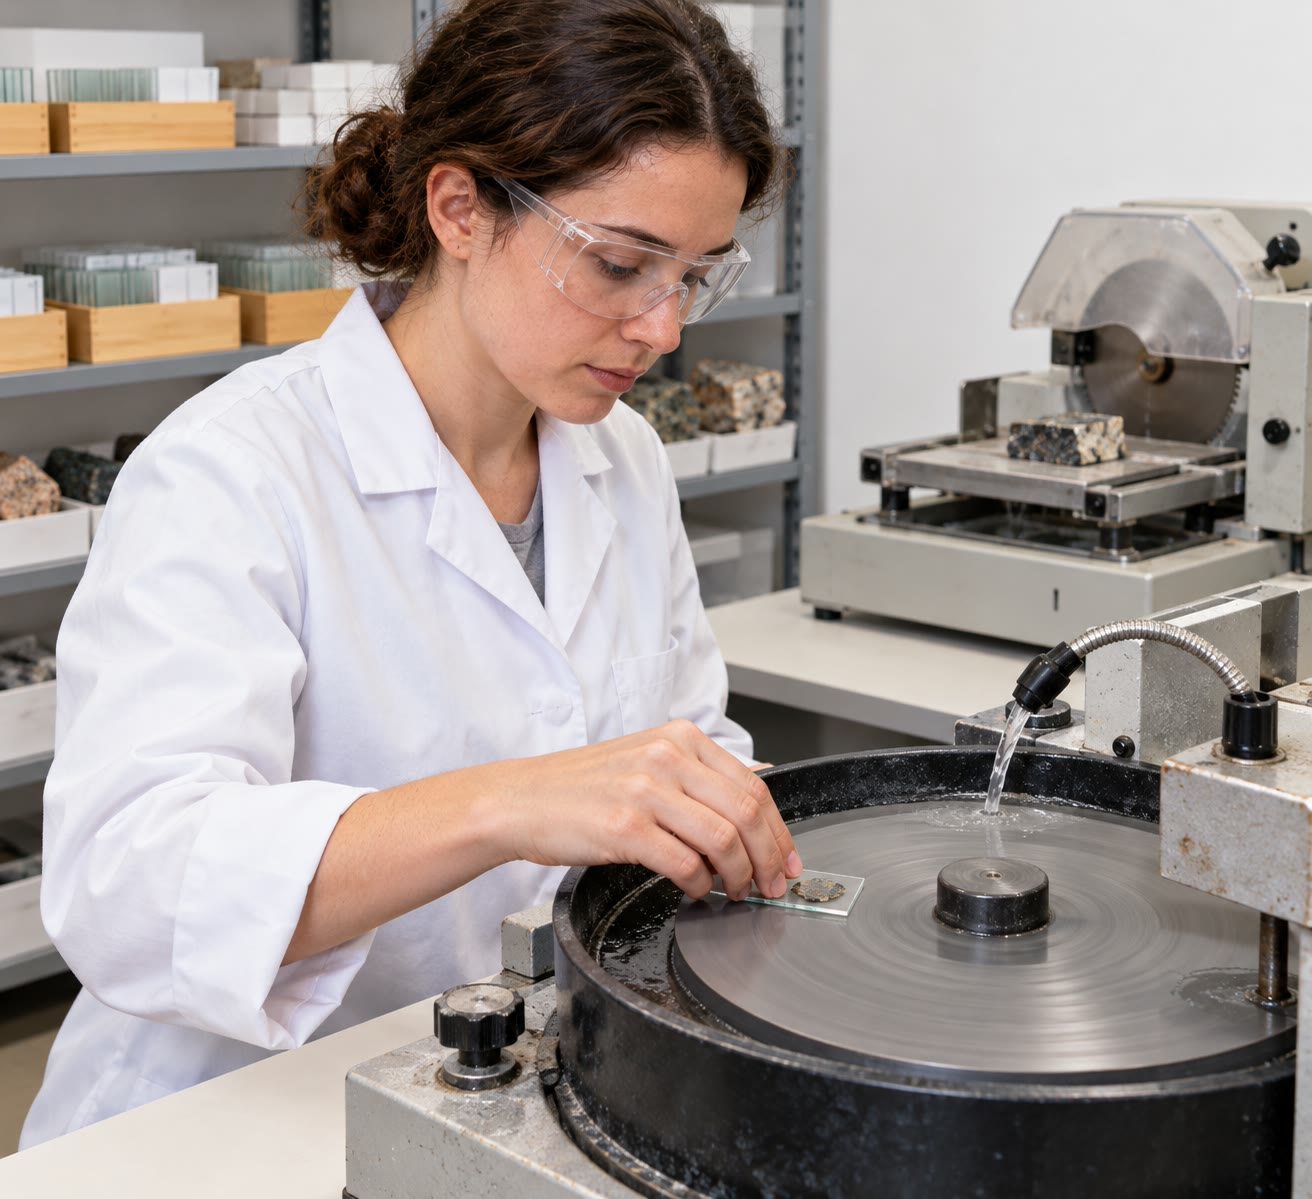
\includegraphics[width=\linewidth]{images/book3/ai/b1-thin-section-lab.jpg}
\end{minipage}
\end{inthelab}

تُدرس \omterm{def:b1:field-lab-methods-1:thin-section}{الشريحة الرقيقة} بمجهر مزوّد بمرشّحين مستقطِبين. والاستقطاب الخطي موضوع الفيزياء: ويكفي هنا أن مرشّحًا مستقطِبًا ينفذ منه الضوء المهتز في اتجاه واحد فقط، وأن مرشّحين متعامدين لا ينفذ منهما أي ضوء.

\begin{definition}[المجهر المستقطِب، والضوء المستقطَب المستوي، والمستقطِبان المتقاطعان]\label{def:b1:field-lab-methods-1:microscope}
\emph{المجهر المستقطِب}\index{المجهر المستقطِب} مجهر بالضوء النافذ، فيه مرشّح مستقطِب (المستقطِب) تحت منضدة تدور بزاوية \ang{360} على مقياس مدرّج، ومرشّح مستقطِب ثانٍ (المحلِّل) بين العدسة الشيئية والعدسة العينية، يمكن إدخاله في مسار الضوء أو إخراجه، واتجاه اهتزازه متعامد على اتجاه المستقطِب. وحين يكون المحلِّل خارج المسار تُرى العينة في \emph{الضوء المستقطَب المستوي}\index{الضوء المستقطَب المستوي}؛ وحين يكون داخله تُرى بين \emph{المستقطِبين المتقاطعين}\index{المستقطِبان المتقاطعان}.
\end{definition}

\begin{omfigure}
\begin{tikzpicture}[font=\scriptsize, x=1cm, y=0.62cm]
\def\comp#1#2#3{\draw[fill=#3] (-1.1,#1-0.18) rectangle (1.1,#1+0.18); \node[right] at (1.3,#1) {#2};}
\draw[omThm!60, line width=3pt, -{Stealth[length=3mm]}] (0,0.3) -- (0,10.6);
\draw[fill=yellow!40] (0,0) circle (0.3); \node[right] at (1.3,0) {مصباح};
\comp{1.3}{المستقطِب: ينفذ اهتزازًا واحدًا فقط}{omDef!25}
\draw[omDef, thick, <->] (-0.5,1.3) -- (0.5,1.3);
\draw[fill=white] (-1.0,2.3) .. controls (0,2.75) .. (1.0,2.3) .. controls (0,1.85) .. (-1.0,2.3);
\node[right] at (1.3,2.3) {المكثِّف};
\draw[fill=black!70] (-1.6,3.4) rectangle (1.6,3.55);
\draw[fill=icsJurassic!40] (-0.5,3.55) rectangle (0.5,3.65);
\node[right] at (1.7,3.48) {منضدة دوّارة، مدرّجة بالدرجات، مع الشريحة الرقيقة};
\draw[fill=white] (-0.45,4.5) rectangle (0.45,5.4); \node[right] at (1.3,4.95) {العدسة الشيئية};
\comp{6.2}{فتحة إضافية}{black!10}
\comp{7.2}{المحلِّل: داخل المسار (مستقطِبان متقاطعان) أو خارجه (ضوء مستقطَب مستوٍ)}{omDef!25}
\draw[omDef, thick, <->] (0,6.85) -- (0,7.55);
\comp{8.2}{عدسة برتراند (اختيارية)}{black!5}
\draw[fill=white] (-0.35,9.1) rectangle (0.35,10.0); \node[right] at (1.3,9.55) {العدسة العينية بخيوط متقاطعة};
\end{tikzpicture}

{\small مسار الضوء في \omterm{def:b1:field-lab-methods-1:microscope}{المجهر المستقطِب} (تخطيطي، من الأسفل إلى الأعلى). المستقطِب والمحلِّل يهتزان متعامدين (السهمان المزدوجان)؛ وإذا لم يكن بينهما شيء، يعطي \omterm{def:b1:field-lab-methods-1:microscope}{المستقطِبان المتقاطعان} مجالًا أسود.}
\end{omfigure}

بين \omterm{def:b1:field-lab-methods-1:microscope}{المستقطِبين المتقاطعين} يبقى زجاج الشريحة، والإيبوكسي، وأي معدن متناحٍ (أي معدن خواصه البصرية واحدة في كل الاتجاهات، كما في البلورات المكعبة) أسود مهما كان دوران المنضدة. وأغلب المعادن ليست متناحية: فهي تغيّر استقطاب الضوء الذي يعبرها، وتظهر بألوان تداخل تتغيّر مع دوران المنضدة، وتختفي أربع مرات في الدورة الكاملة. ولماذا تفعل ذلك، وكيف تُعرّف الألوان والزوايا معدنًا، فموضوع \cref{ch:b1:optical-mineralogy}. وتُفحص المعادن في \omterm{def:b1:field-lab-methods-1:thin-section}{الشريحة الرقيقة} عادةً بتكبيرات من نحو $16\times$ إلى $400\times$.
% ledger: jaic:magnification

\begin{omfigure}
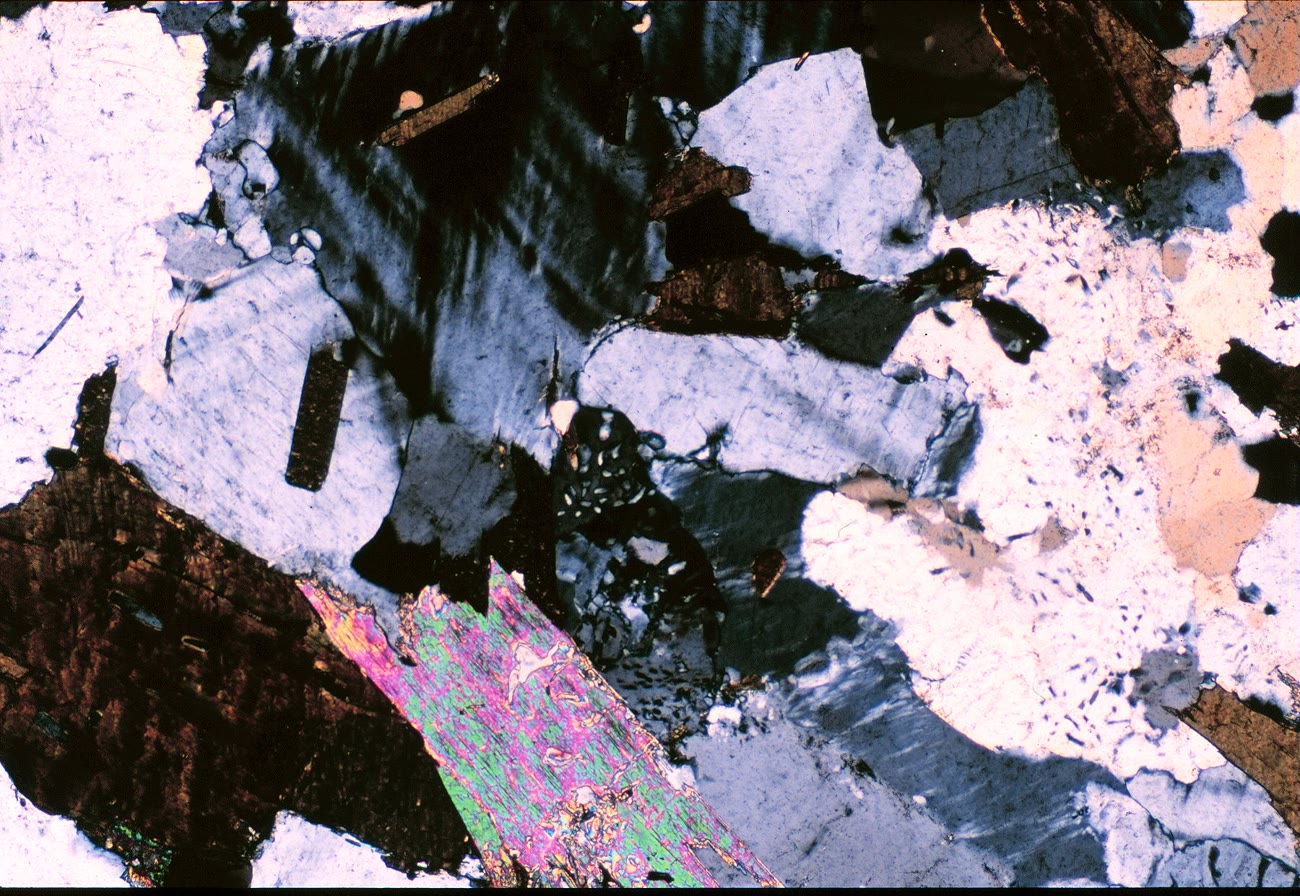
\includegraphics[width=0.55\linewidth]{images/book3/b1-granite-thin-section-xpl.jpg}
% ledger: commons:granite-xpl

{\small صخر جرانيتي في \omterm{def:b1:field-lab-methods-1:thin-section}{الشريحة الرقيقة} بين \omterm{def:b1:field-lab-methods-1:microscope}{المستقطِبين المتقاطعين}. البيوتيت بني، والموسكوفيت يُظهر ألوان تداخل وردية وخضراء زاهية، والبلاجيوكلاز مخطَّط بتوأمه، والكوارتز أبيض إلى رمادي. الصورة: Darla Sondrol، بترخيص CC0 (Wikimedia Commons).}
\end{omfigure}

\begin{safety}
العمل الحقلي والمخبري يُجعل آمنًا بقواعد مهنية، لا بالحظ. ففي الحقل يعمل الجيولوجيون اثنين اثنين، أو يتركون خطة مكتوبة لطريقهم وساعة عودتهم؛ ويحملون توقعات الطقس والخرائط وإسعافات أولية، ويبتعدون عن قاع الجروف وحافاتها ووجوه المحاجر، ويضعون الخوذة ووقاية العين حيثما يمكن للصخر أن يسقط أو يتشظّى؛ والعمل في المواقع النشطة يتبع قواعد المشغّل. وفي المختبر تعمل المناشير والأقراص الدوّارة خلف واقيات مع الماء لتخفيف الغبار، وتُعالَج الراتنجات والأحماض بالقفازات والنظارات تحت شفاطة، ولكل مادة كيميائية ورقة بيانات السلامة الخاصة بها. ولا يخص أيّ من هذه الأنشطة قارئ هذا الكتاب وحده: فالفصل يصف الممارسة المهنية.
\end{safety}

\section{التمارين}

\begin{exercise}[$\star$]\label{exo:b1:field-lab-methods-1:1}
يعطي جهاز استقبال الأقمار الصناعية مواضع دقيقة ضمن نحو \qty{4.9}{m}. كم تكون هذه المسافة على خريطة بمقياس 1:10\,000؟ وعلى مقياس 1:25\,000؟
\end{exercise}

\begin{exercise}[$\star$]\label{exo:b1:field-lab-methods-1:2}
تقرأ بوصلة بلا ضبط للانحراف \omterm{def:b1:geological-maps:attitude}{اتجاه الانحدار} \ang{052} على طبقة. أعطِ \omterm{def:b1:geological-maps:attitude}{اتجاه الانحدار} الجغرافي إذا أُجريت القراءة في ريكيافيك في 1 يناير 2026، ثم في ويلينغتون في اليوم نفسه (الصندوق المؤرَّخ).
\end{exercise}

\begin{exercise}[$\star$]\label{exo:b1:field-lab-methods-1:3}
ينغمس محور \omterm{def:b1:geological-maps:fold}{طية} بزاوية \ang{20} نحو \ang{015}. اكتب اتجاهه كما في النص، وأعطِ متجهة وحدته الهابطة بمركبات شرقية وشمالية وعلوية.
\end{exercise}

\begin{exercise}[$\star$]\label{exo:b1:field-lab-methods-1:4}
ثلاث قراءات لمفصل شاقولي تعطي أسمات ناظمه \ang{350} و\ang{358} و\ang{006}. احسب وسطها الحسابي، ثم سمت محصلة المتجهات الأفقية الوحدوية الثلاث. أيّ المتوسطين صحيح؟
\end{exercise}

\begin{exercise}[$\star\star$]\label{exo:b1:field-lab-methods-1:5}
خمس قراءات لانحدار طبقة واحدة هي \ang{34} و\ang{37} و\ang{35} و\ang{33} و\ang{36}. احسب متوسطها، وانحرافها المعياري، والخطأ المعياري للمتوسط.
\end{exercise}

\begin{exercise}[$\star\star$]\label{exo:b1:field-lab-methods-1:6}
يأخذ جيولوجي قراءة على كل جناح من \omterm{def:b1:geological-maps:fold}{طية} متماثلة: $090/30$ و$270/30$. احسب المتوسط المتجهي و$\bar R$. ما الخطأ الذي وقع؟
\end{exercise}

\begin{exercise}[$\star\star$]\label{exo:b1:field-lab-methods-1:7}
خدوش على سطح تطبّق وضعيته $080/12$ لها اتجاه \ang{120}. ما غوصها؟ وما يكون إذا كان الاتجاه \ang{170}؟
\end{exercise}

\begin{exercise}[$\star\star$]\label{exo:b1:field-lab-methods-1:8}
في إدنبرة يكون الانحراف المغناطيسي \ang{-0.47} في 1 يناير 2026، ويتغيّر بمقدار \ang{+0.20} في السنة. إذا افترضنا أن التغيّر يبقى ثابتًا، فمتى يبلغ الصفر، وما قيمته في 1 يناير 2030؟
\end{exercise}

\begin{exercise}[$\star\star$]\label{exo:b1:field-lab-methods-1:9}
ثلاث قراءات لطبقة واحدة هي $080/10$ و$080/12$ و$080/14$. بيّن أن متوسطها المتجهي هو $080/12$، واحسب $\bar R$ والتقدير $\sqrt{2(1 - \bar R)}$ لتقدير $\theta_{\text{جذر المتوسط}}$، وقارنه بالزاوية الجذرية المتوسطة المضبوطة.
\end{exercise}

\begin{exercise}[$\star\star\star$]\label{exo:b1:field-lab-methods-1:10}
تقطع \omterm{def:b1:field-lab-methods-1:thin-section}{الشريحة الرقيقة} حبيبة كروية نصف قطرها $r$ على بُعد $h$ من مركزها، مع احتمال تساوي $h$ في أي موضع بين 0 و$r$. بيّن أن متوسط نصف قطر الدائرة المرئية في الشريحة هو $\pi r/4$. ما متوسط حجم حبيبات كوارتز عرضها \qty{0.50}{mm} كما تبدو في \omterm{def:b1:field-lab-methods-1:thin-section}{الشريحة الرقيقة}؟
\end{exercise}

\begin{exercise}[$\star\star\star$]\label{exo:b1:field-lab-methods-1:11}
بيّن أنه إذا زيد كل اتجاه انحدار في مجموعة من القراءات بالزاوية نفسها $D$، فإن \omterm{def:b1:geological-maps:attitude}{اتجاه الانحدار} للمتوسط المتجهي يزيد بالمقدار $D$، وانحداره لا يتغيّر. لماذا يهمّ ذلك في تصحيح الانحراف المغناطيسي؟
\end{exercise}

\begin{exercise}[$\star\star\star$]\label{exo:b1:field-lab-methods-1:12}
على طبقة تنحدر بزاوية \ang{12}، ينتشر ناظم قراءة واحدة بانحراف معياري قدره \ang{2} في كل من اتجاهين متعامدين: على طول خط \omterm{def:b1:geological-maps:attitude}{الانحدار} الأشدّ، وهو ما يغيّر \omterm{def:b1:geological-maps:attitude}{الانحدار}، وعبره، وهو ما يغيّر \omterm{def:b1:geological-maps:attitude}{اتجاه الانحدار}. كم قراءة تلزم لخطأ معياري قدره \ang{0.5} في متوسط \omterm{def:b1:geological-maps:attitude}{الانحدار}؟ و\ang{1} في متوسط \omterm{def:b1:geological-maps:attitude}{اتجاه الانحدار}؟
\end{exercise}

\section{مسألة: موسم حقلي على الجناح الشرقي لفاردن}

\begin{problem}[{مسألة نهاية الأسبوع --- متوسط اثنتي عشرة قراءة بوصلة، وقياس تشتّتها، وتصحيحها، ومقارنتها بالآبار}]
\label{pb:b1:field-lab-methods-1:1}
% readings: figdata/bachelor-1/attitude_stats.py (part normals); values: calc/ch06.py
قاس جيولوجي \omterm{def:b1:geological-maps:attitude}{وضعية} طبقات الجناح الشرقي \omterm{def:b1:geological-maps:fold}{لطية} فاردن المحدبة في اثنتي عشرة محطة، بوصلة مضبوطة على الانحراف، مقرِّبًا إلى الدرجة. ويعطي الجدول كل قراءة (\omterm{def:b1:geological-maps:attitude}{اتجاه الانحدار}/\omterm{def:b1:geological-maps:attitude}{الانحدار}) ومركبات ناظمها الوحدوي نحو الأعلى $\vec n = (n_E, n_N, n_U)$، مقرّبةً إلى أربع منازل عشرية.
\begin{center}
\small
\begin{tabular}{rcccc@{\qquad}rcccc}
\hline
 & القراءة & $n_E$ & $n_N$ & $n_U$ & & القراءة & $n_E$ & $n_N$ & $n_U$ \\
\hline
\mbox{\textdir TLT 1} & $076/11$ & \mbox{\textdir TLT 0.1851} & \mbox{\textdir TLT 0.0462} & \mbox{\textdir TLT 0.9816} & \mbox{\textdir TLT 7} & $083/11$ & \mbox{\textdir TLT 0.1894} & \mbox{\textdir TLT 0.0233} & \mbox{\textdir TLT 0.9816} \\
\mbox{\textdir TLT 2} & $081/13$ & \mbox{\textdir TLT 0.2222} & \mbox{\textdir TLT 0.0352} & \mbox{\textdir TLT 0.9744} & \mbox{\textdir TLT 8} & $083/12$ & \mbox{\textdir TLT 0.2064} & \mbox{\textdir TLT 0.0253} & \mbox{\textdir TLT 0.9781} \\
\mbox{\textdir TLT 3} & $078/16$ & \mbox{\textdir TLT 0.2696} & \mbox{\textdir TLT 0.0573} & \mbox{\textdir TLT 0.9613} & \mbox{\textdir TLT 9} & $085/12$ & \mbox{\textdir TLT 0.2071} & \mbox{\textdir TLT 0.0181} & \mbox{\textdir TLT 0.9781} \\
\mbox{\textdir TLT 4} & $081/11$ & \mbox{\textdir TLT 0.1885} & \mbox{\textdir TLT 0.0298} & \mbox{\textdir TLT 0.9816} & \mbox{\textdir TLT 10} & $078/11$ & \mbox{\textdir TLT 0.1866} & \mbox{\textdir TLT 0.0397} & \mbox{\textdir TLT 0.9816} \\
\mbox{\textdir TLT 5} & $076/10$ & \mbox{\textdir TLT 0.1685} & \mbox{\textdir TLT 0.0420} & \mbox{\textdir TLT 0.9848} & \mbox{\textdir TLT 11} & $081/13$ & & & \\
\mbox{\textdir TLT 6} & $083/14$ & \mbox{\textdir TLT 0.2401} & \mbox{\textdir TLT 0.0295} & \mbox{\textdir TLT 0.9703} & \mbox{\textdir TLT 12} & $082/11$ & & & \\
\hline
\end{tabular}
\end{center}

\medskip
\noindent\textbf{الجزء الأول --- \omterm{def:b1:field-lab-methods-1:mean-orientation}{الوضعية المتوسطة}.}
\begin{enumerate}
  \item احسب الأوساط الحسابية لاتجاهات \omterm{def:b1:geological-maps:attitude}{الانحدار} الاثني عشر، ولانحداراتها الاثني عشر.
  \item أعطِ مثالًا لقراءتين يكون فيهما المتوسط الحسابي لاتجاهي \omterm{def:b1:geological-maps:attitude}{الانحدار} عبثيًا، وبيّن لماذا يكون آمنًا هنا.
  \item بيّن أن $\vec n = (\sin\delta\sin\alpha, \sin\delta\cos\alpha,
        \cos\delta)$ متجهة وحدوية عمودية على خط \omterm{def:b1:geological-maps:attitude}{الانحدار} وعلى خط \omterm{def:b1:geological-maps:attitude}{الامتداد} للمستوي $\alpha/\delta$.
  \item أكمل الجدول للقراءتين 11 و12.
  \item احسب المحصلة $\vec S$ للنواظم الاثني عشر.
  \item احسب $\|\vec S\|$ وطول المحصلة المتوسط $\bar R$.
  \item استنتج المتوسط المتجهي: اتجاه انحداره وانحداره.
\end{enumerate}

\medskip
\noindent\textbf{الجزء الثاني --- تشتّت القراءات.}
\begin{enumerate}[resume]
  \item احسب الانحرافات المعيارية للعينة لاتجاهات \omterm{def:b1:geological-maps:attitude}{الانحدار} ولانحدارات.
  \item باستعمال \cref{prop:b1:field-lab-methods-1:vector-mean}، قدّر الجذر المتوسط لمربع الزاوية $\theta_{\text{جذر المتوسط}}$ بين القراءات ومتوسطها، بالدرجات.
  \item توقّع $\theta_{\text{جذر المتوسط}}$ من الانحرافين المعياريين في السؤال 8 وصيغة الخطأ في الفصل، ثم قارن.
  \item أيّ الانحرافين المعياريين يسهم أكثر في $\theta_{\text{جذر المتوسط}}$، ولماذا؟
  \item احسب الأخطاء المعيارية لمتوسط \omterm{def:b1:geological-maps:attitude}{الانحدار} ولمتوسط \omterm{def:b1:geological-maps:attitude}{اتجاه الانحدار}.
  \item هل تشتّت اتجاهات \omterm{def:b1:geological-maps:attitude}{الانحدار}، أي \ang{2.9}، علامة على قياس مهمل؟ علّل.
\end{enumerate}

\medskip
\noindent\textbf{الجزء الثالث --- الانحراف المغناطيسي.}
\begin{enumerate}[resume]
  \item نسي جيولوجي ثانٍ ضبط الانحراف. وقد أعطت قراءاتها الاثنتا عشرة المتوسط المتجهي $083.1/12.1$ في أسمات مغناطيسية. افترض أن الانحراف المغناطيسي في تلال فاردن في تلك السنة يبلغ \ang{2.5} غربًا. ما متوسطها في أسمات جغرافية؟
  \item لماذا يكون متوسط انحدارها صحيحًا دون تصحيح؟
  \item هل كان بإمكانها أن تصحّح كل قراءة قبل أخذ المتوسط، بدلًا من تصحيح المتوسط؟ وهل يغيّر ذلك الجواب (\cref{exo:b1:field-lab-methods-1:11})؟
  \item بعد عشر سنين، يعيد طالب استعمال ضبطها للانحراف، بينما تغيّر الانحراف بمقدار \ang{0.2} في السنة. ما حجم الخطأ، مقارنةً بالخطأ المعياري في السؤال 12؟
  \item أعطِ امتداد \omterm{def:b1:field-lab-methods-1:mean-orientation}{الوضعية المتوسطة} للجيولوجي الأول وفق قاعدة اليد اليمنى.
\end{enumerate}

\medskip
\noindent\textbf{الجزء الرابع --- البوصلة والآبار.}
\begin{enumerate}[resume]
  \item من ثلاث آبار، وجد \cref{ch:b1:geological-maps} \omterm{def:b1:geological-maps:attitude}{الوضعية} $080.6/12.2$ لقاعدة الحجر الجيري. قارنها بالمتوسط المتجهي للسؤال 7، زاوية بزاوية.
  \item احسب الزاوية بين الناظمين.
  \item الخطأ المعياري لاتجاه المتوسط نحو $\theta_{\text{جذر المتوسط}}/\sqrt N$. هل الفرق في السؤال 20 دالّ إحصائيًا؟
  \item كم قراءة تلزم لتقليل ذلك الخطأ المعياري إلى النصف؟
  \item اذكر خطأين لا يقلّلهما أي عدد من القراءات.
  \item أعطِ \omterm{def:b1:field-lab-methods-1:mean-orientation}{الوضعية المتوسطة} للجناح الشرقي من القراءات الاثنتي عشرة، على صورة \omterm{def:b1:geological-maps:attitude}{اتجاه الانحدار}/\omterm{def:b1:geological-maps:attitude}{الانحدار} مقرَّبة إلى الدرجة.
\end{enumerate}
\end{problem}
